\section{Introduction}
\label{sec:intro}

The Named-data Link State Routing protocol (NLSR) is an intra-domain routing protocol for Named Data Networking (NDN).
It is an application level protocol similar to many IP routing protocols, but NLSR uses NDN's Interest/Data packets to disseminate routing updates.
Although NLSR is designed in the context of a single domain, its design patterns may offer a useful reference for future development of inter-domain routing protocols.

NLSR supports name-based routing in NDN, computes routing ranks for all policy-compliant next-hops which provides a name-based multi-path routing table for NDN's forwarding strategy,
and ensures that routers can originate only their own routing updates using a hierarchical trust model.

\subsection{NLSR Modules and Data Structures}
\label{sec:modules}
NLSR contains multiple modules that each contribute to the total realization of the protocol.
Many of the modules interact with one another to trigger some behavior or to modify information in data structures.
NLSR uses the following modules:
\begin{itemize}
\item \textbf{Hello Protocol} (Section~\ref{sec:hello-protocol}) - determines the status of neighboring routers using periodic Hello Interests and notifies other modules when neighbors' statuses change.
\item \textbf{NSync} - provides LSDB synchronization by extending the ChronoSync protocol~\cite{chronosync}.
\item \textbf{Sync Logic Handler} (Section~\ref{sec:sync-logic}) - handles sync update notifications from NSync by retrieving updated LSAs.
\item \textbf{LSAs} (Section~\ref{sec:lsas}) - represent routing information published by the router.
\item \textbf{LSDB} (Section~\ref{sec:lsdb}) - stores the LSA information distributed by other routers in the network.
\item \textbf{Routing Table} (Section~\ref{sec:routing-table}) - calculates and maintains a list of next hops for each router in the network.
\item \textbf{Name Prefix Table} (Section~\ref{sec:npt}) - stores all advertised name prefixes and their next hops.
\item \textbf{FIB} (Section~\ref{sec:fib}) - maintains a shadow FIB which represents the intended state of NFD's FIB~\cite{NFD}.
\item \textbf{Prefix Update Processor} - listens for dynamic prefix announcements to advertise or withdraw name prefixes.
\end{itemize}

\subsection{Protocol Overview}
\label{sec:protocol-overview}

NLSR is designed to accomplish three main tasks: (1) discover adjacent neighbors; (2) disseminate and synchronize topology, name prefix, and hyperbolic routing information; and (3) calculate a consistent routing table and populate NFD's FIB.
The entire protocol is described in detail in the NLSR paper~\cite{NlsrTr}.

\subsubsection{Discovering Neighbors}

NLSR determines the adjacency status of neighboring routers using the Hello Protocol module (Section~\ref{sec:hello-protocol}).
When the Hello Protocol detects a status change for a neighbor, it will ask the LSDB module (Section~\ref{sec:lsdb}) to update the router's advertised adjacency information.

\subsubsection{Disseminating Routing Information}

When one of a router's LSAs (Section~\ref{sec:lsas}) changes, the information of this change should be distributed to every other router in the network.
The Sync Logic Handler module (Section~\ref{sec:sync-logic}) is used to notify the synchronization protocol of changes to the router's own LSAs as well as to learn of LSA changes from other routers in the network;
the Sync Logic Handler module interfaces with NSync to perform the two tasks.

When the Sync Logic Handler module learns of a new LSA, it will inform the LSDB module.
The LSDB module will attempt to fetch the new LSA and will store it in the LSDB module's database if it can be retrieved.
If the newly fetched LSA informs the router of previously unknown routing information, the LSDB module will inform other modules depending on the type of routing information:
\begin{itemize}
\item \textbf{Change in network topology} - the LSDB module will inform the Routing Table module (Section~\ref{sec:routing-table}), so the Routing Table module can calculate an up-to-date routing table.
\item \textbf{Change in name prefix advertisement} - the LSDB module will inform the Name Prefix Table module (Section~\ref{sec:npt}), which will in turn notify the FIB module (Section~\ref{sec:fib}) in order to add or remove the changed name prefixes.
\item \textbf{Change in hyperbolic coordinates} - the LSDB module will inform the Routing Table module (Section~\ref{sec:routing-table}), so the Routing Table module can calculate an up-to-date routing table.
\end{itemize}

\subsubsection{Calculating the Routing Table and Populating NFD's FIB}

When the routing table is calculated by the Routing Table module, the computed next hops are passed to the Name Prefix Table module.
The Name Prefix Table module will then further pass the next hops to the FIB module to update NLSR's expected state of NFD's FIB.
The FIB module will then perform the registrations or unregistrations with NFD's FIB.\\

A simplified diagram of NLSR's actions when receiving new routing information is shown in Figure~\ref{fig:system-interaction}.
The remainder of this documentation will describe the purpose of and interaction between each module in more detail.

\begin{figure}
\center
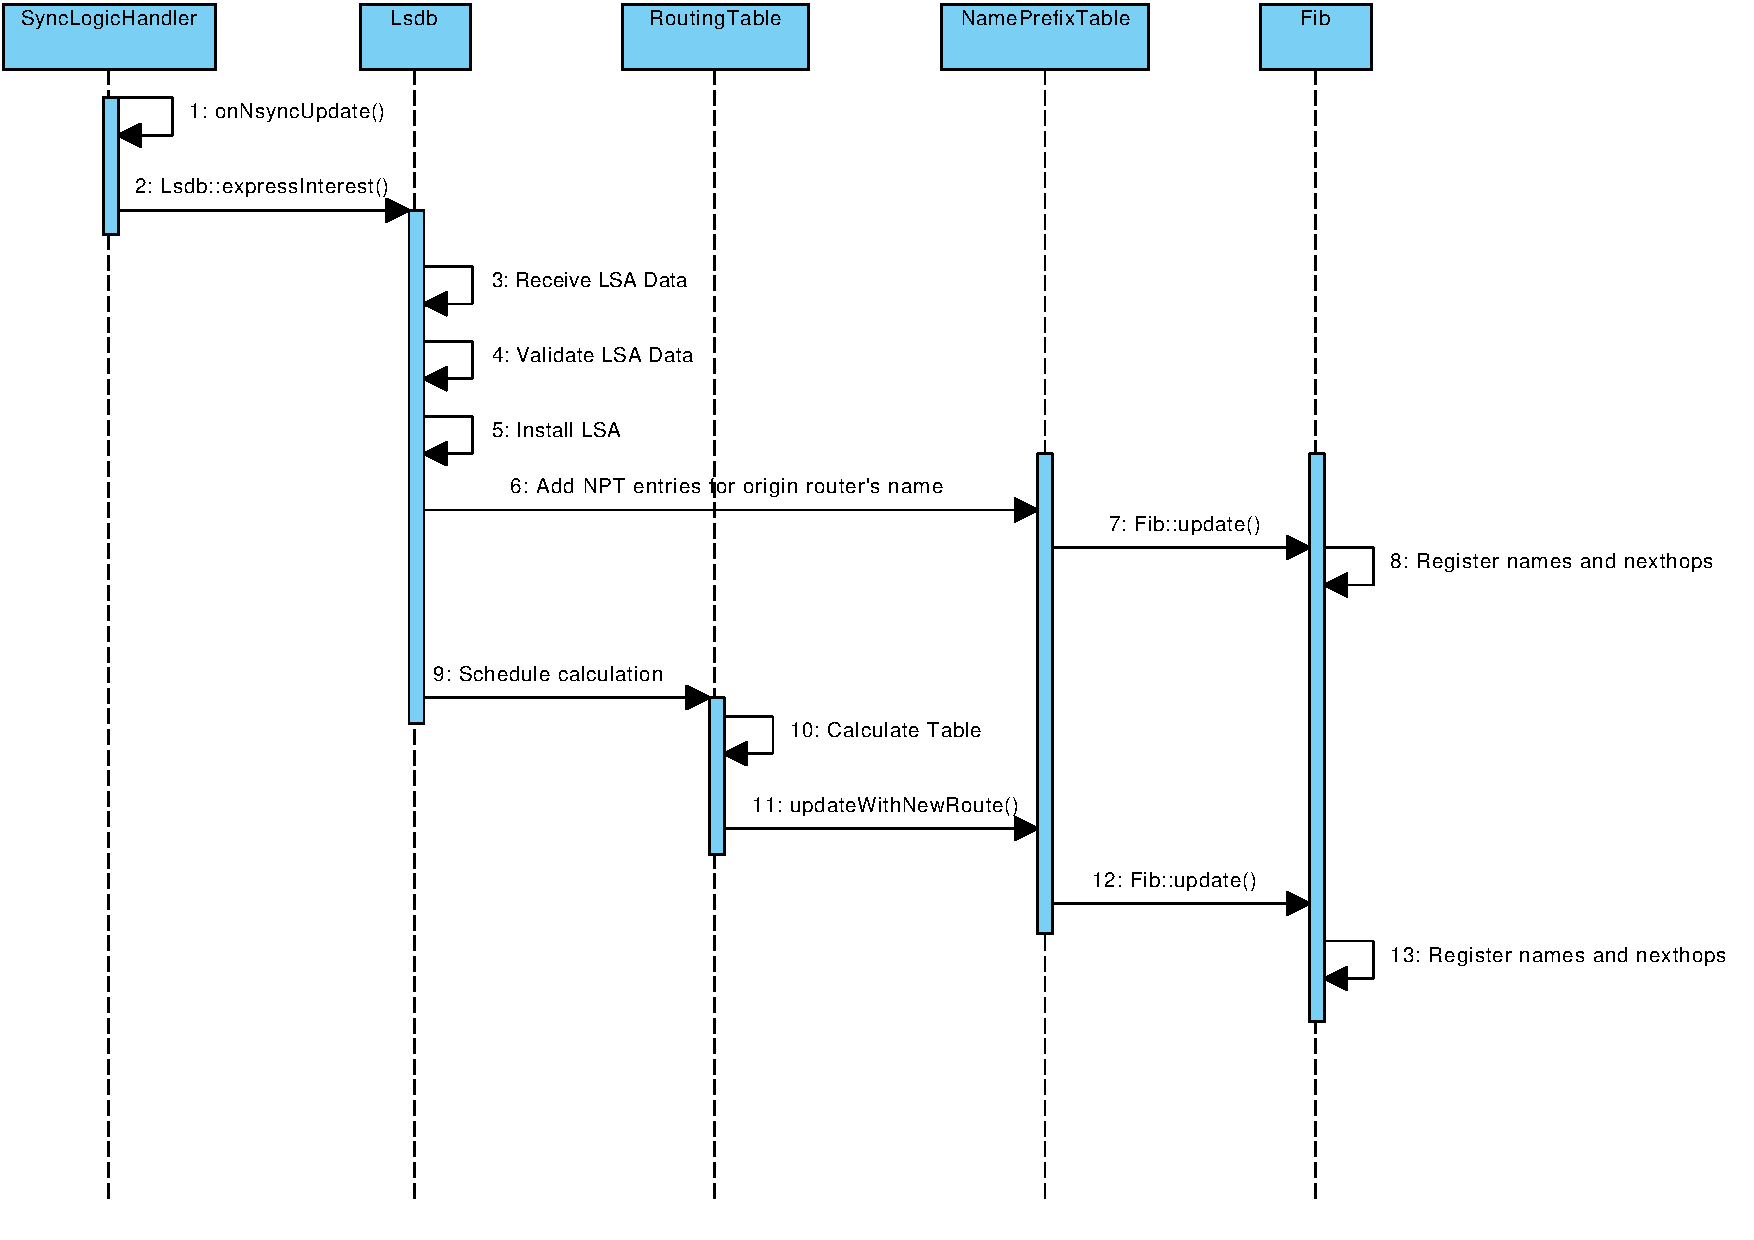
\includegraphics[width=\linewidth]{figures/system-interaction.pdf}
\caption{Simplified Diagram of the Actions of NLSR's Modules}
\label{fig:system-interaction}
\end{figure}

